%!TEX root = ../report.tex
\section{Implementation}
\label{sec:impl}
The solution that has been proposed in the previous section is implemented using the C++ programming language in combination with the OpenGL API.
To program on the GPU, Cg is used as shading language.

The actual SPH fluid simulation is given and can be seen in figure \ref{fig:sph}, by implementing the multiple passes described in the previous section, a nature like fluid is expected.
By creating Frame Buffer Objects (FBO), the results can be written to an off-screen rendering target.
This is useful since we are using multiple passes.
Also, multiple buffers can be attached to the FBO.

\subsection{Depth determination}
The depth at each fragment of each particle closest to the camera is determined using a combination of a vertex- and fragment shader.
Each particle has a position in world space that is passed to the vertex shader.
These particles are rendered as spheres to determine the correct depth values.

The vertex shader computes and passes the following properties of each particle to the fragment shader:
\begin{itemize}
 	\item Position of center in eye space.
 	\item Position of center in screen space.
 	\item Splat size.
 	\item Splat radius.
 \end{itemize} 

The fragment shader uses this input to determine the depth at every fragment.
To determine this depth, the splat is rendered as a sphere by discarding fragments that fall outside the sphere.
From this, the normal from the center of the sphere towards its surface is determined by taking the difference of the current fragment position and the current particle center.
Using this normal, the point is transformed to clip space, the $z$ value of this position is the depth value.
The depth values are then written to the depth buffer of the current FBO.

The depth component of each fragment can be visualized as grey value by setting the R, G and B components to the depth value.
The results of this visualization can be seen in figure \ref{fig:depth}.
It can be observed that the particles become darker when they appear  closer to the camera.

\begin{figure}[!th]
\hrule
\begin{center}
\vspace*{2ex}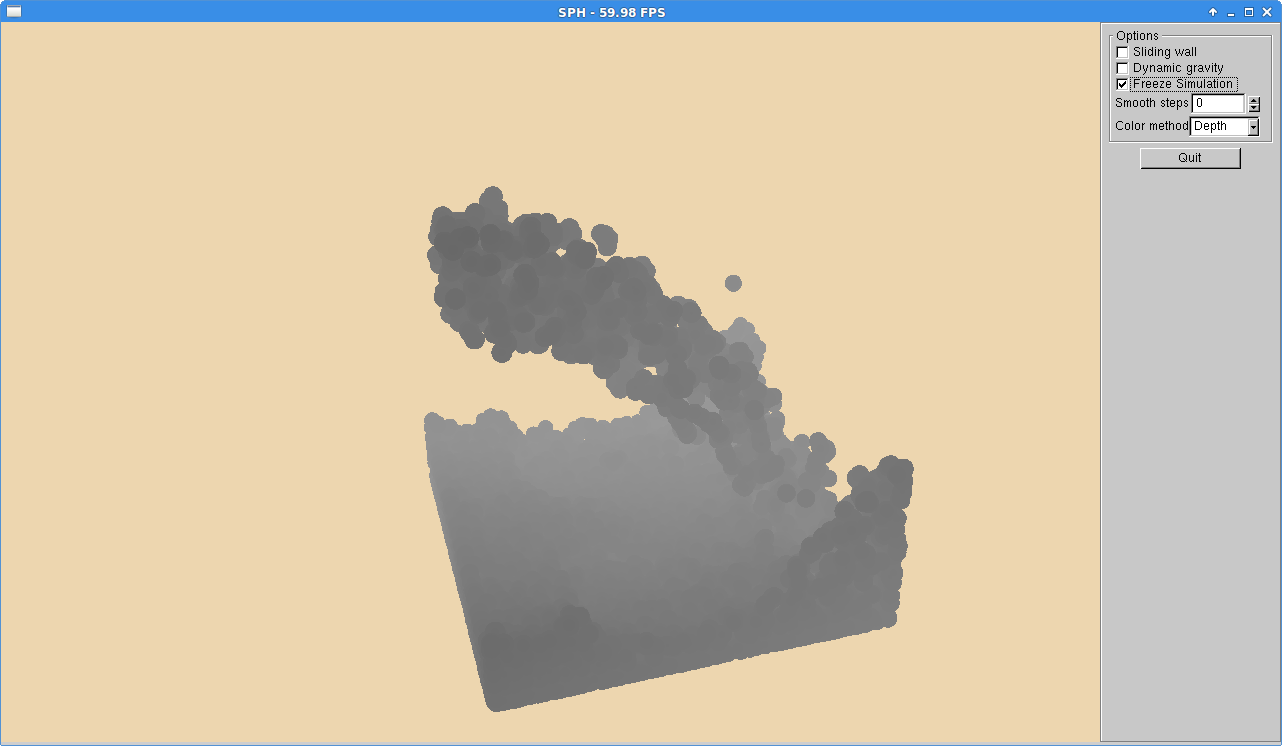
\includegraphics[width=0.48\textwidth,clip=true,trim=10cm 1cm 10cm 3cm]{pictures/depth_normal.png}
\end{center}
\caption{Visualisation of the depth components}
\label{fig:depth} 
\vspace*{2ex}
\hrule
\end{figure}



\subsection{Surface smoothing}
Smoothing is done using a fragment shader.
% For the smoothing of the surface there is one fragment shader with two depth textures.
The original depth values are modified using curvature flow to smooth the surface.
Since one cannot modify the depth texture that is used for reading, there are two depth textures which are alternated during computation.

The smoothing is determined in multiple iterations and depth values are modified in several timesteps.
% For the smoothing the normals do not have to be explicitly calculated, .
In pseudocode, the algorithm is as follows.
% Two fragment shaders are used for surface smoothing.
% The first fragment shader calculates the surface normals from the depth values and writes them in a texture.
% The second fragment shader smooths the depth values using curvature flow, using the surface normals computed in the first shader.
% These smoothed depth values are also written to a texture.

% Since the smoothing happens in multiple steps, and textures can not be overwritten directly, multiple textures and FBOs are needed.
% The depth texture has to be updated, so an extra temporary depth texture is needed, the same holds for the surface normal texture.
% In each smooth step, one texture is used as input and the other is used as render target, the textures are switched after every step.
% The surface normals change when the depth values are changed, so these also need to be recomputed every smooth step.
% Listing \ref{program:smooth} shows this process in pseudocode.

\begin{algorithm}
	\begin{program}
	\caption
	\FOR i:=1 \TO |smoothSteps| \DO
		|smoothDepths()|;
		|flipTextures()|;
	\end{program}
	\label{program:smooth}
	\caption{Surface smoothing pseudocode}
\end{algorithm}


\subsubsection{Depth smoothing}
Using the depth values, finite differencing can be applied to determine derivatives of these values to obtain the curvature in every point, as equation~\ref{eq:curvy} describes.
This curvature is used to modify the depth values which are subsequently written to another depth texture.
We had trouble implementing this step in Cg, but we found a reference \footnote{\url{https://github.com/halcy/simpleflow/blob/master/WaterSim2/curvatureflow.frag}} that implemented the smoothing in GLSL, which we adapted to our needs.

\subsection{Rendering}
For the final rendering phase we implemented a fragment shader that produces a color for each fragment, which only has a depth component.
We have a default color - RGB(0.02, 0.1, 0.3), with $\alpha = 0.5$ - for a fluid that is modified according to its surroundings based on shading. 
The end-results are projected onto a full-screen quad, which is the best option due to our framebuffer-objects.

The paper suggests to implement a combination of Phong shading and the Fresnel equation for displaying the surface. 
Normally, computing the Fresnel equation would be a costly and difficult operation.
To circumvent this, we have applied Schlick's approximation to determine the reflective Fresnel component \cite{schlick1994inexpensive}.

\subsubsection{Normal calculation}
To determine the normals of the surface, the depth buffer is passed as input to the fragment shader, along with the uniform variables $C_x$ and $C_y$.
Since the depth buffer is in a texture, we can obtain the depth values of neighbors.
Using these neighbors, the finite differences between depth values can be calculated in the $x$ and $y$ direction.
Since we now have $C_x, C_y, \frac{\partial z}{\partial x}, \frac{\partial z}{\partial y}$ and $z$, we can approximate the normals according to equation \ref{eq:normals}.
A visualization of the normals, done by assigning the normal to the color output, can be seen in figure~\ref{fig:normals} and \ref{fig:normals2}. 
These normals are essential for a correct shading of the surface, but are not explicitly needed for the smoothing of the surface.


\begin{figure}[!th]
\hrule
\begin{center}
\vspace*{2ex}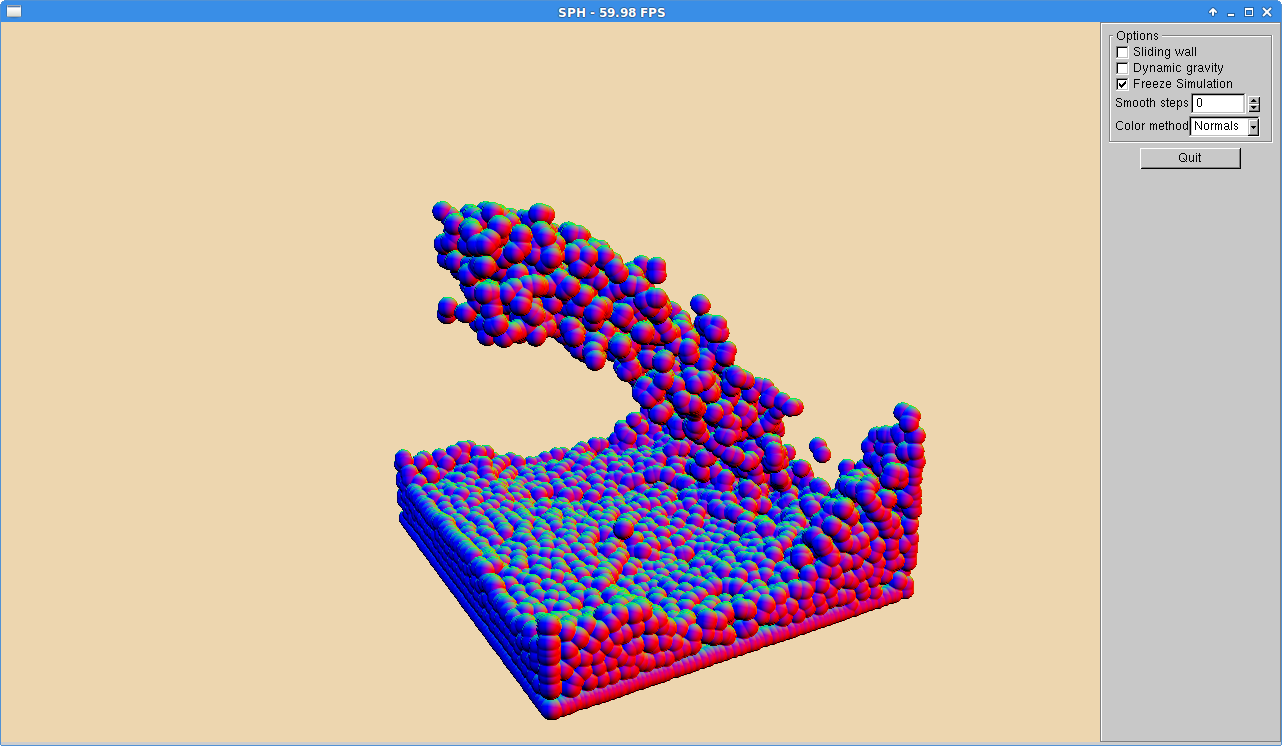
\includegraphics[width=0.48\textwidth,clip=true,trim=10cm 1cm 10cm 3cm]{pictures/normal_normal.png}
\end{center}
\caption{Visualization of the normals of a unsmoothed surface}
\label{fig:normals} 
\vspace*{2ex}
\hrule
\end{figure}

\begin{figure}[!th]
\hrule
\begin{center}
\vspace*{2ex}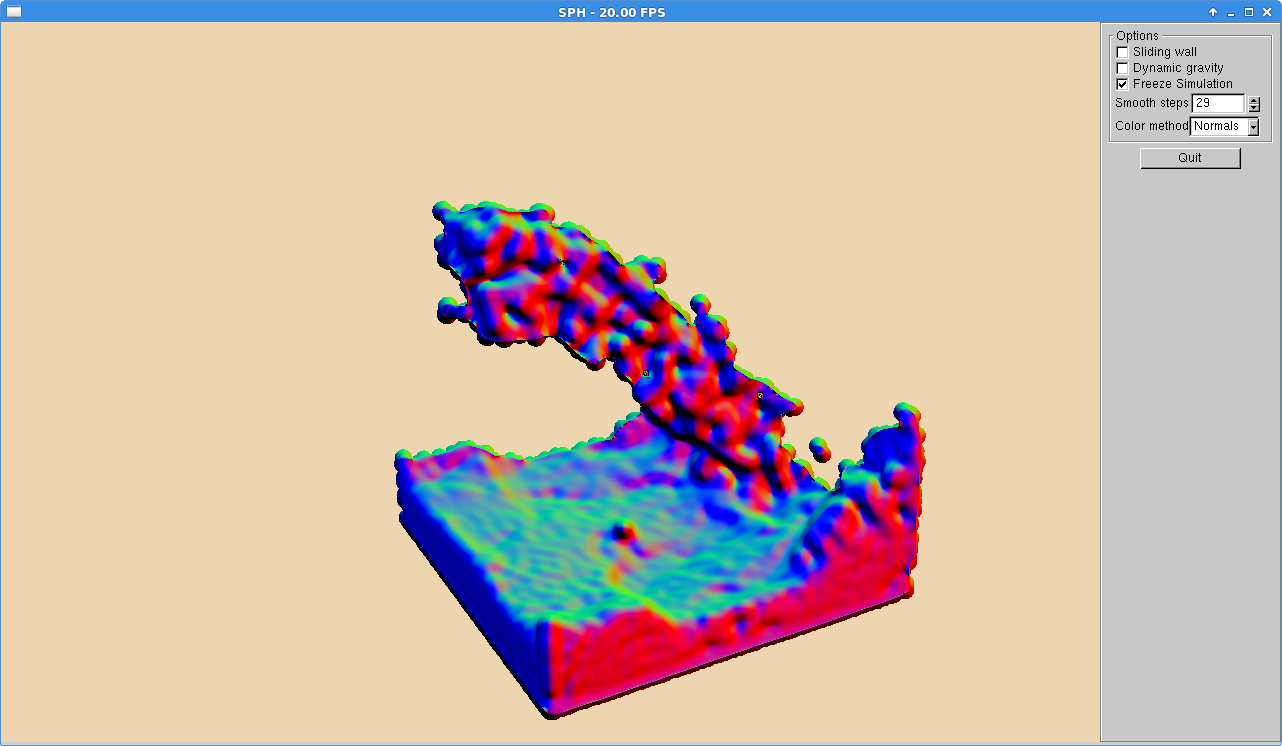
\includegraphics[width=0.48\textwidth,clip=true,trim=10cm 1cm 10cm 3cm]{pictures/normals_smoothed.png}
\end{center}
\caption{Visualization of the normals of a smoothed surface}
\label{fig:normals2} 
\vspace*{2ex}
\hrule
\end{figure}